\section{Introduction}
\seclabel{introduction}

Consider a robot fulfilling orders in a warehouse.
The robot must quickly plan grasps for consumer products to fullfill orders.
Furthermore, the robot may not precisely know the state of the environment, such as the pose or frictional properties of object, due to sensor imprecision and missing data (e.g. occlusions in point clouds).
This poses a challenge for many existing grasp planning methods that are based on precise knowledge of contact locations and surface normals~\cite{ciocarlie2009, ferrari1992} due to the distribution on possible environment configurations.

In vision and speech, advances in Big Data and distributed computing, combined with datasets of milliions of examples such as ImageNet~\cite{deng2009imagenet} and the Fisher corpus~\cite{cieri2004fisher}, have produced impressive results~\cite{hannun2014deepspeech, hays2008im2gps, krizhevsky2012imagenet} that surpass those obtained from decades of research on analytic methods.
This raises the question: will machine learning of grasps for vast numbers of possible object poses, object shapes, environment configurations, etc., exhibit scaling effects similar to those observed in computer vision and speech recognition?

\begin{figure}[t!]
\centering
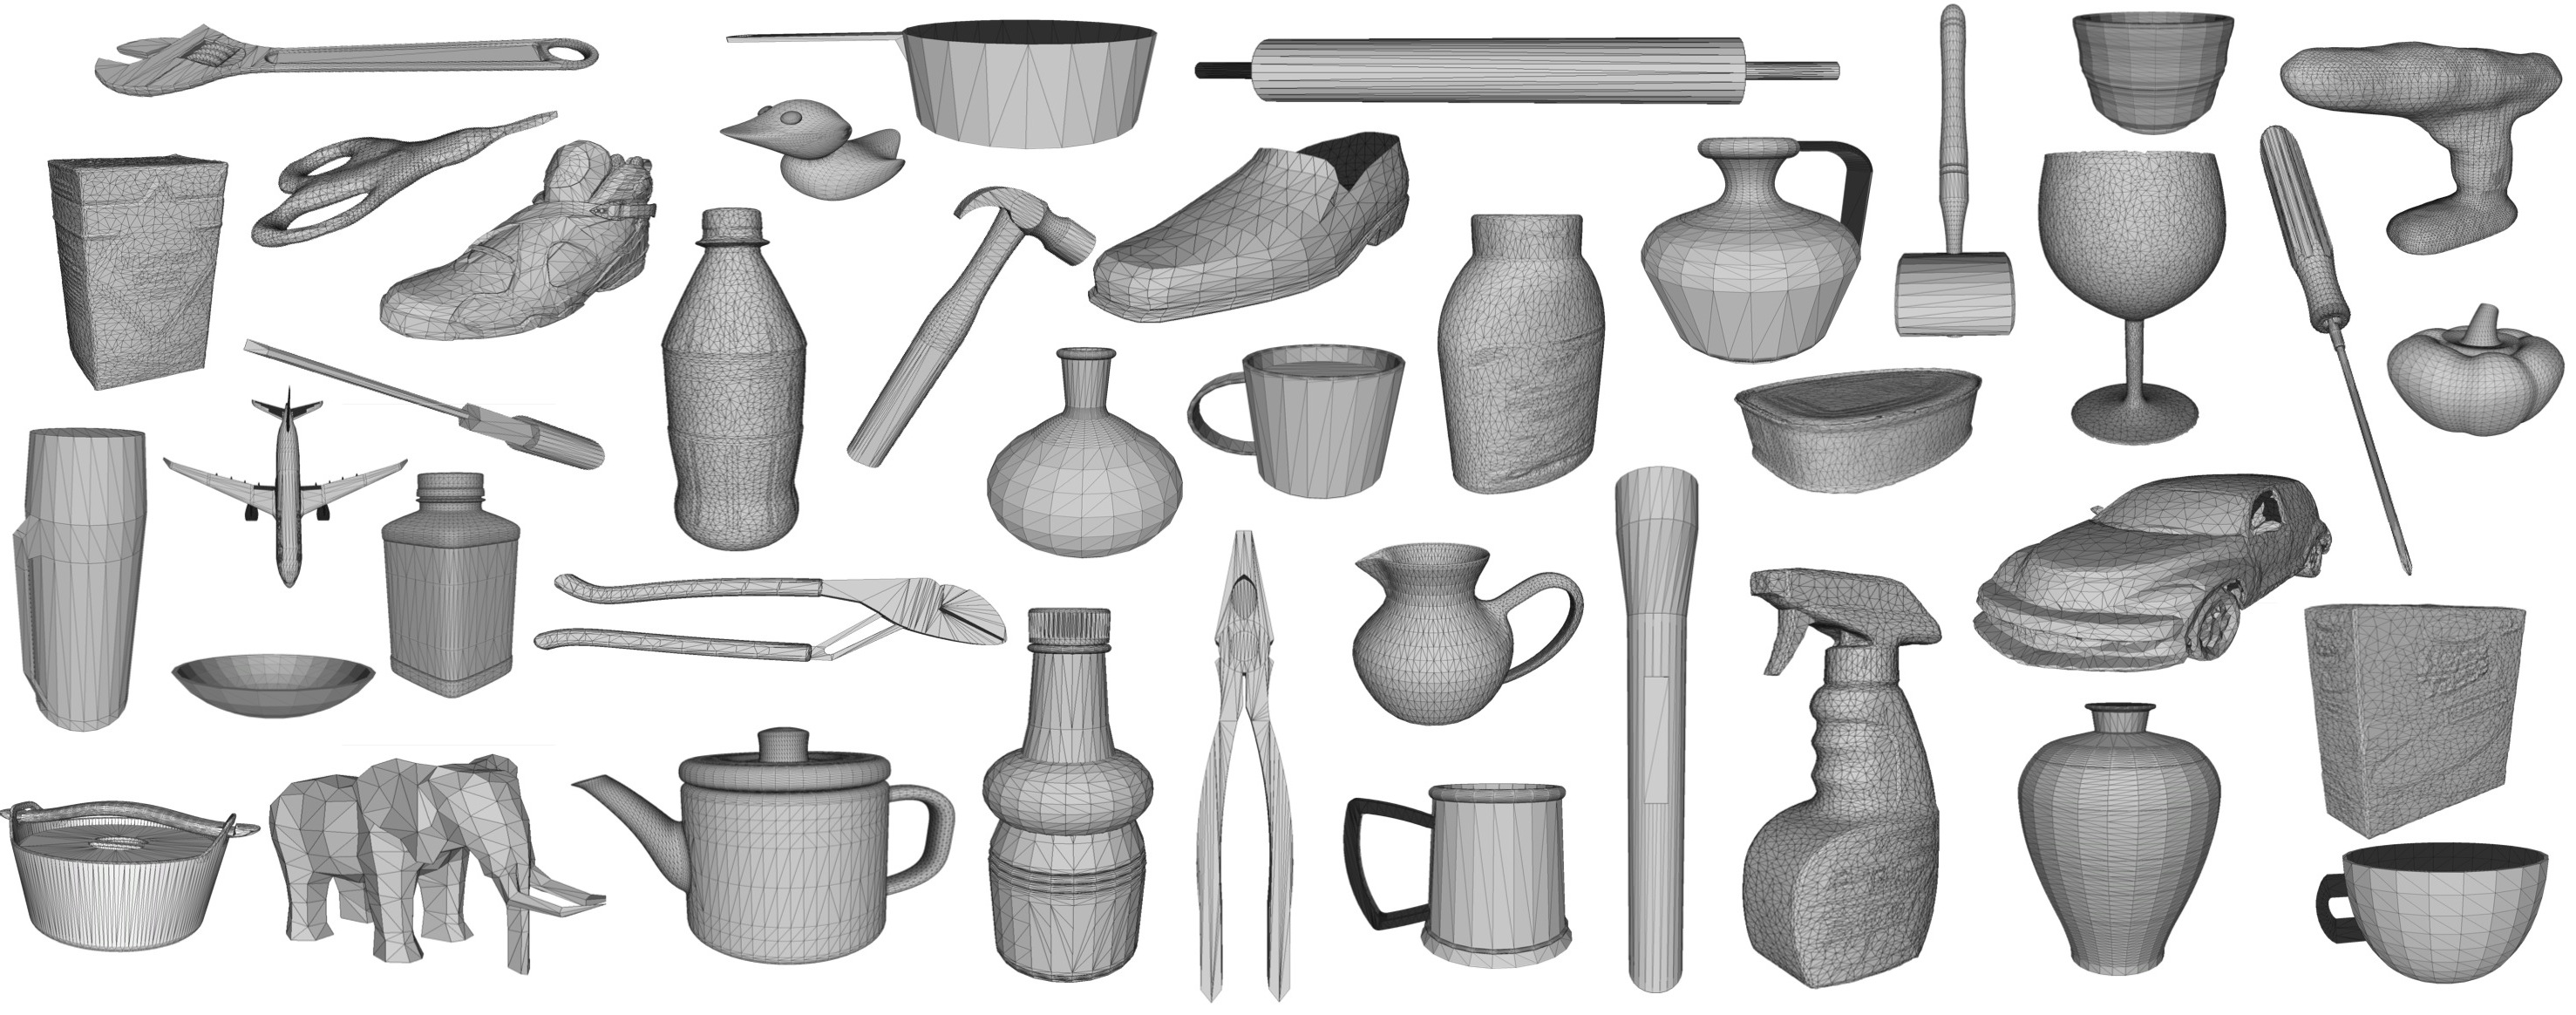
\includegraphics[scale=0.085]{figures/dexnet_collage.jpg}
\caption{Sample of 3D mesh models from the Dex-Net dataset. The dataset currently includes over 10,000 models from laser-scanned datsets such as the KIT object database~\cite{kasper2012kit} and the Yale-CMU-Berkeley object set~\cite{calli2015benchmarking}, and synthetic datasets such as 3DNet\cite{wohlkinger20123dnet}, ModelNet~\cite{wu20143d}, and the SHREC 2014 object retrieval challenge dataset~\cite{li2015comparison}. }
\figlabel{dexnet-teaser}
\vspace*{-15pt}
\end{figure}

We introduce Dex-Net 1.0, a dataset of 3D models and grasps with similarity metrics, and a system for actively acquiring statistical models of grasp quality across the network.
The Dex-Net dataset contains representative 3D models of objects that could be encountered in warehousing or the home.
Dex-Net contains laser-scanned 3D mesh models from the KIT object database~\cite{kasper2012kit}, the Amazon Picking Challenge objects, BigBIRD~\cite{singh2014bigbird}, and YCB ~\cite{calli2015benchmarking} to reflect physical objects commonly used for benchmarking in grasping research.
The dataset also includes synthetic 3D mesh models from shape classification datasets such as 3DNet~\cite{wohlkinger20123dnet}, ModelNet~\cite{wu20143d}, and the SHREC 2014 large scale object retrieval challenge~\cite{li2015comparison} to scale the number of models.
~\figref{dexnet-teaser} shows a sample of the objects in the dataset.
We measure object similarity based the distance between feature vectors generated from multi-view Convolutional Neural Networks (CNNs)~\cite{su2015multi}, a state-of-the are method in shape retrieval
We measure similarity between grasps by the pose of the gripper and local surface ``heightmaps" extracted at location of contact with an object~\cite{herzog2012template, kappler2015leveraging}.
Our system uses Google Cloud Platform to distribute grasp quality evaluations across hundreds of virtual machines and to store millions of grasps across the objects in Dex-Net.

In this work, we use Dex-Net to study the convergence rate of Multi-Armed Bandit (MAB) algorithms for finding a grasp with high probability of force closure under object pose, gripper pose, and friction coefficient uncertainty from a set of 250 candidate grasps on objects from Dex-Net.
To do so, we extend the MAB framework of Laskey et al.~\cite{laskey2015bandits} to model correlations between the probability of force closure for similar grasps on similar 3D objects using Continuous Correlated Beta Processes (CCBPs)~\cite{goetschalckx2011continuous, montesano2012active}.
CCBPs predict a belief distribution for the quality of each grasp based similarity to data in Dex-Net that can be efficiently updated after observing the quality of a grasp for a sampled object pose, gripper pose, and friction coefficient.
Our results suggest that CCBPs bootstrapped with data from Dex-Net can accelerate grasp planning by up to $10\times$.


 





